\chapter{Resultados y discusión}
\label{chap:resultados}

% Versión 4: incorpora los resultados y la discusión del OE2 y la parte sustentada del
% OE3 (muografia-documentada, rama principal 08cdc0c: revisión EF-01-C2, síntesis del
% OE2 y curvas descriptivas de exposición). Cifras generadas desde los JSON del repositorio.
% Versión 3: incorpora los resultados y la discusión del OE1 (campaña de 114 vistas).
% Cifras contrastadas con la entrega f395570 de muografia-documentada y con las
% revisiones de la dirección (c4e467f, efeee44, 58f9c12 y 4529c49).

Este capítulo presenta los resultados obtenidos con los procedimientos del capítulo~\ref{chap:metodologia} y su interpretación. Se organiza en tres secciones, una por objetivo específico: el conjunto de datos sintéticos, su calidad y su reproducibilidad (OE1); los ensayos de desarrollo del modelo y su evaluación final (OE2), y el análisis descriptivo del desempeño frente a la exposición (OE3). En cada una se mantiene la distinción de la metodología entre resultados confirmatorios, descriptivos y exploratorios, y se indica el criterio con el que se interpreta cada resultado. Los resultados de los objetivos segundo y tercero sobre las particiones reservadas tienen carácter descriptivo, porque esas escenas habían sido evaluadas en una etapa anterior del proyecto (sección~\ref{subsec:met-protocolo}).

% =============================================================================
\section{Conjunto de datos sintéticos del OE1}
\label{sec:res-oe1}

Los resultados de esta sección proceden de la campaña de 114 vistas ejecutada entre el 2 y el 3 de octubre de 2026 y de los ensayos que la precedieron. Todas las cifras se obtuvieron de los registros, inventarios y evaluaciones conservados en el repositorio de referencia, y las de la campaña se contrastaron, además, con la revisión directa de la dirección, que repitió la evaluación desde los histogramas y regeneró los pares de forma independiente. La exposición sigue el orden de la cadena: primero los ensayos previos, después la ejecución y la integridad de la campaña, luego los dos indicadores de calidad de las referencias y, por último, la discusión del producto obtenido.

\subsection{Resultados de los ensayos previos a la campaña}
\label{subsec:res-ensayos}

Las comprobaciones del generador confirmaron la normalización de la fuente. La escala $S_0$ recalculada directamente desde la parametrización de Guan difirió de la tabla en $6{,}2\times10^{-5}$ en términos relativos, y la prueba $\chi^2$ de la distribución de direcciones por filas de elevación, con 255 grados de libertad, dio valores de 290,4, 224,3 y 265,1 en tres simulaciones independientes, con valores $p$ aproximados de 0,06, 0,92 y 0,32; sumada sobre una imagen completa, la relación de la \cref{eq:fuente-t} reprodujo el conteo total con un cociente de 1,00014.

Los ensayos de la corrección geométrica mostraron que la regla B1 eliminó las advertencias de superposición en los controles ejecutados, sin evidencia de un cambio en los conteos que la estadística disponible pudiera resolver. El piloto A/B sobre geo-train-06 resultó inconcluso, como se había anticipado en su prerregistro por falta de potencia en la región de intersección. La primera etapa del segundo ensayo, con 1\,300\,000 transportes de producción incluida la repetición técnica, dio una diferencia estimada nula en la región de interés en ambas geometrías, con un intervalo diagnóstico de aproximadamente $\pm12{,}8$ cuentas por millón de primarios, y su repetición A/A fue idéntica byte a byte a la referencia; sin embargo, solo un muon de producción cruzó la región de intersección, sin llegar al detector, y los cruces sintéticos de control entraron todos desde el cuerpo denso, de modo que no se contrastó la entrada desde el conducto. El complemento dirigido cubrió esa situación: la variante corregida asignó la región compartida al cuerpo denso en los 36 pares de trayectorias, mientras que la variante original la asignó al conducto en los 18 casos dirigidos desde ese lado; tres pares cambiaron de píxel y ninguno cambió su detección. La segunda etapa, con el tamaño fijado de antemano, estimó una diferencia de $+0{,}125$ detecciones por millón de primarios con un intervalo conservador del 95\,\% de $[-0{,}229;\ +0{,}469]$ por millón, de modo que su resultado fue inconcluso: no demostró equivalencia dentro del margen ni una diferencia relevante fuera de él, y el diseño no preveía ampliar el tamaño. La auditoría independiente de sus registros superó 6\,966 controles sin fallos.

Los controles del observable fijaron la receta de producción. Con la inyección 1~m antes de la roca y el umbral de 3~GeV, la razón de conteos entre los planos de 100 y 600~m fue, por bandas de espesor másico de roca, de 1,000, 0,999, 0,994, 0,990 y 0,991, con un mínimo de $0{,}9895\pm0{,}0025$, y ese umbral conservó el 83,5\,\% del conteo en roca; entre los planos de 600 y 1\,200~m la diferencia fue nula. La misma inyección elevó la eficiencia de cielo abierto, sin umbral, al 99,97\,\% de media, con una fila mínima de 99,69\,\%; la variante intermedia fijada de antemano no había cumplido el criterio, y la inyección junto a la roca se añadió después y se evaluó con el mismo criterio. En los bordes, ninguna configuración cumplió el criterio estricto de los controles cortos: con la inyección junto a la roca y un margen de 5°, el sesgo medio desapareció ($-0{,}07$ puntos porcentuales) y la desviación máxima fue de 1,65 puntos porcentuales, de modo que ese control quedó abierto y su verificación se trasladó al criterio de bordes de la campaña. Con los datos anidados, solo entre el 3,6 y el 70,4\,\% de los registros del plano de 600~m, según la banda de espesor, cayeron dentro del panel de 1,2~m, lo que confirma que la convergencia entre planos grandes no informa sobre la equivalencia con el panel. La integración de la malla angular, con 1\,000 primarios, produjo 750 registros y superó sus controles de metadatos, histograma, registro y código de salida.

Por último, el piloto de seis vistas, con $2{,}11\times10^{8}$ primarios por vista, completó sus 36 bloques sin fallos y sus 90 regiones de borde quedaron dentro de la tolerancia de $\pm1$ punto porcentual. En la roca, la mediana fue de 121 a 127 cuentas por región y entre el 63 y el 65\,\% de las regiones alcanzó 100 cuentas. Con esas tasas, una proyección binomial a $3{,}44\times10^{8}$ primarios estimó una fracción media de regiones con al menos 100 cuentas de 89,7 a 91,1\,\% para esa geometría; la proyección no garantizaba el 90\,\% en todas las vistas, y así quedó registrado en el acuerdo previo a la campaña.

\subsection{Ejecución e integridad de la campaña}
\label{subsec:res-campana}

La campaña se ejecutó entre el 2 de octubre de 2026 a las 18:10:27 y el 3 de octubre a las 09:48:49, unas 15,6 horas de reloj. La \cref{tab:ejecucion} resume su ejecución. Los 1\,026 bloques del manifiesto terminaron y se publicaron verificados; tres trabajos, correspondientes a las filas 120 a 122, fallaron porque se agotó la cuota de almacenamiento del directorio personal en el clúster, se conciliaron con los registros del gestor y se completaron en un reintento, sin que ninguna fila quedara con más de una ejecución completada. La fusión, la evaluación, la exportación y el inventario terminaron sin errores.

\begin{table}[htbp]
\centering
\caption[Ejecución de la campaña de 114 vistas]{Ejecución de la campaña de 114 vistas. Fuente: elaboración propia a partir de los registros del gestor de trabajos y de los metadatos de la fusión del repositorio de referencia.}
\label{tab:ejecucion}
\small
\begin{tabularx}{\linewidth}{@{}lX@{}}
\toprule
Elemento & Valor \\
\midrule
Primarios & $3{,}44\times10^{8}$ por vista; $3{,}9216\times10^{10}$ en total, en 1\,026 bloques \\
Trabajos & 1\,029: 1\,026 completados y 3 fallidos por cuota de almacenamiento, reintentados y completados \\
Duración por bloque & 128,9~s de media; mínimo 105~s y máximo 161~s \\
Recursos asignados & 2\,356,73 hilo-horas, incluidos los trabajos fallidos \\
Direcciones nominales en la ventana & de 235\,330\,375 a 235\,366\,529 por vista \\
Muones registrados con $E_k>3$~GeV & de 115\,272\,159 a 121\,975\,257 por vista; $1{,}3546\times10^{10}$ en total \\
Exposición convencional, $T_v$ & de 195,92 a 195,95 días convencionales por vista \\
\bottomrule
\end{tabularx}
\end{table}

La integridad del producto se verificó en los tres niveles previstos. Las 114 referencias resultaron técnicamente completas, sin vistas faltantes ni errores, con los primarios, las semillas, la receta, las geometrías y las tablas del manifiesto. Las huellas de los 248 archivos de la fusión y de los 229 archivos de la exportación coincidieron con sus inventarios, y las 114 imágenes exportadas conservaron exactamente los conteos y las coordenadas de los histogramas; la suma de los conteos de las imágenes coincidió con la de los muones registrados en los metadatos. La revisión de la dirección repitió la evaluación desde los histogramas con el plan, la receta y las máscaras congelados y obtuvo las mismas decisiones y valores, con una diferencia máxima entre números de coma flotante de $4{,}97\times10^{-14}$ frente a una tolerancia de $10^{-10}$.

Los 9\,120 pares se regeneraron dos veces de forma independiente, en una segunda máquina de los estudiantes y en la revisión de la dirección, en ambos casos con NumPy 2.4.4. En las dos regeneraciones coincidieron las 342 huellas de contenido de las referencias, las entradas y las fracciones de los 114 archivos; ningún conteo reducido superó a su referencia y ningún valor se recortó. Las huellas de los archivos comprimidos, en cambio, difirieron entre máquinas, porque dependen de la versión de la biblioteca de compresión, lo que confirma la necesidad de comparar el contenido y no solo los archivos. La copia de distribución, con 753 archivos y 1\,126\,769\,406 bytes, se recuperó desde su enlace con una cuenta distinta de la propietaria y coincidió archivo por archivo con los inventarios; la dirección la verificó de nuevo de forma independiente, con 2\,291 controles satisfactorios.

La \cref{fig:res-referencias} muestra seis de las 114 referencias, elegidas para ilustrar el control homogéneo, los tres tipos de anomalía, una combinación de los tres y dos de las vistas que quedaron por debajo de la meta de roca. En todas, el cielo y la silueta del edificio están bien definidos, y la roca presenta conteos de varios órdenes de magnitud menores que el cielo abierto.

\begin{figure}[htbp]
\centering
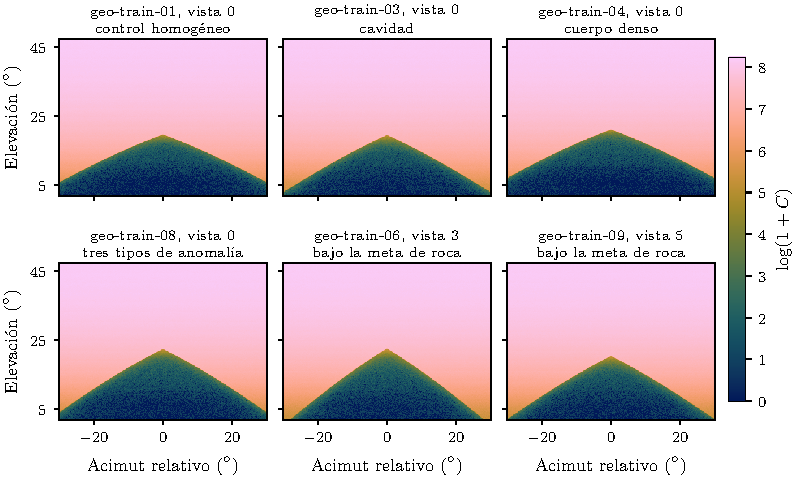
\includegraphics{fig4-1_referencias.pdf}
\caption[Seis referencias de la campaña de 114 vistas]{Seis referencias de la campaña de 114 vistas, en la escala común $\log(1+C)$, donde $C$ es el conteo del píxel, sin suavizado. Las vistas se eligieron para ilustrar casos y no constituyen una muestra estadística; las siluetas no son mapas de densidad. Fuente: elaboración propia a partir de las imágenes exportadas de la campaña, verificadas contra su inventario de huellas.}
\label{fig:res-referencias}
\end{figure}

\subsection{Respuesta en los bordes de la ventana}
\label{subsec:res-bordes}

Las 1\,710 regiones de borde, quince por cada una de las 114 vistas, resultaron equivalentes según el criterio de la \cref{eq:bordes}: el intervalo completo de su contraste quedó dentro de $\pm1$ punto porcentual, con una cobertura simultánea de la familia de al menos 95\,\%. La \cref{fig:res-bordes} presenta los 1\,710 intervalos agrupados por región. El extremo más alejado de cero fue de 0,933 puntos porcentuales, en la columna~2 de la vista~5 de geo-train-02. Los intervalos de las filas superiores son más estrechos que los de las columnas laterales, porque cada fila abarca toda la anchura de la ventana a la mayor elevación y reúne, por ello, más muones que una columna restringida a la banda de cielo de 30° a 42°.

\begin{figure}[htbp]
\centering
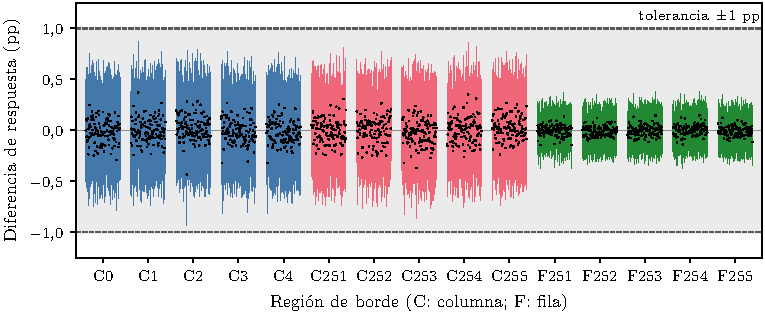
\includegraphics{fig4-2_bordes.pdf}
\caption[Respuesta en las regiones de borde de las 114 vistas]{Intervalos simultáneos del contraste de respuesta $\Delta_r$ (\cref{eq:bordes}) en las quince regiones de borde de cada una de las 114 vistas, en puntos porcentuales: columnas extremas izquierdas (C0 a C4) y derechas (C251 a C255) y filas superiores (F251 a F255). Cada segmento es una vista y cada punto, su estimación central; la franja gris marca la tolerancia de $\pm1$ punto porcentual. Fuente: elaboración propia a partir de la evaluación de la campaña.}
\label{fig:res-bordes}
\end{figure}

\subsection{Suficiencia del conteo en roca}
\label{subsec:res-roca}

El indicador descriptivo de la \cref{eq:roca} alcanzó la meta de 0,90 en 107 de las 114 vistas. La \cref{fig:res-roca} lo presenta por geometría y vista y lo relaciona con el número de regiones de roca de cada vista. Por vista, la fracción de regiones con al menos 100 cuentas varió entre 0,892 y 1,000, con una mediana de 0,961; la mediana de cuentas por región, entre 190 y 260,5, y el percentil 10, entre 97,2 y 157,5. Sobre el total de la campaña, 20\,713 de las 21\,816 regiones evaluadas alcanzaron 100 cuentas, es decir, el 94,944\,\%. Esa proporción global es descriptiva: no sustituye el indicador por vista ni convierte las siete excepciones en cumplimientos.

\begin{figure}[htbp]
\centering
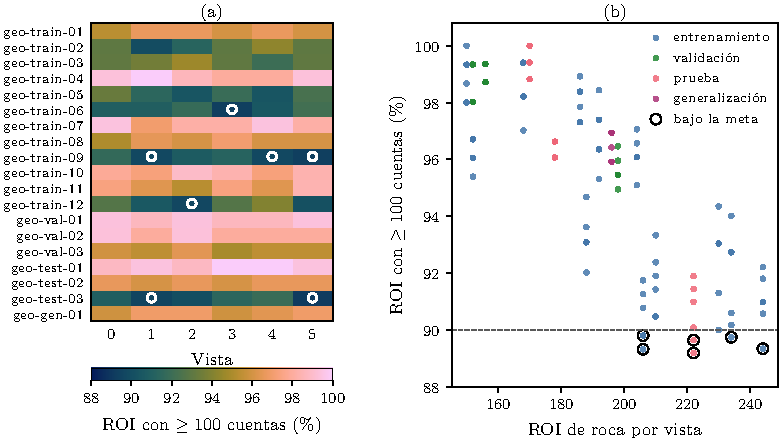
\includegraphics{fig4-3_roca.pdf}
\caption[Suficiencia del conteo en roca por vista]{Indicador descriptivo de suficiencia del conteo en roca (\cref{eq:roca}). (a)~Porcentaje de regiones de roca de $4\times4$ píxeles con al menos 100 cuentas, por geometría y vista; los círculos señalan las vistas por debajo de la meta del 90\,\%. (b)~El mismo porcentaje frente al número de regiones de roca de la vista, por partición; la línea discontinua marca la meta. Fuente: elaboración propia a partir de la evaluación de la campaña.}
\label{fig:res-roca}
\end{figure}

Las siete vistas por debajo de la meta, que la \cref{tab:excepciones} detalla, se conservaron sin cambios, conforme al acuerdo previo: no se aumentó el número de primarios, no se descartaron imágenes ni se modificó la regla después de conocer los resultados. Las siete comparten tres rasgos documentados. En primer lugar, todas quedaron a una o dos regiones de alcanzar la meta: con entre 206 y 244 regiones por vista, les faltaron una o dos regiones con 100 cuentas para llegar al 90\,\%. En segundo lugar, su percentil 10 se situó entre 97,2 y 100,0 cuentas, es decir, el déficit se concentra en un pequeño grupo de regiones con conteos próximos al umbral, y no en regiones sin señal. En tercer lugar, pertenecen a cuatro de las seis geometrías con más regiones de roca por vista, entre 206 y 244 frente a una mediana de 192 en el catálogo, lo que indica una mayor extensión de la banda de espesor nominal evaluada. Ese último rasgo no basta como explicación, porque las otras dos geometrías de ese grupo, geo-train-02, con 230 regiones, y geo-train-05, con 210, alcanzaron la meta en sus seis vistas, con mínimos de 0,900 y 0,905. El repositorio no establece una causa física individual para cada excepción; su cercanía al umbral es compatible con las fluctuaciones de conteo de las regiones próximas a 100 cuentas, sin que esa compatibilidad se haya demostrado con un análisis específico.

\begin{table}[htbp]
\centering
\caption[Vistas por debajo de la meta descriptiva de roca]{Vistas por debajo de la meta descriptiva de roca. $M_v$: regiones de roca de la vista; $n_{\geq100}$: regiones con al menos 100 cuentas; $F_v$: indicador de la \cref{eq:roca}; faltan: regiones adicionales necesarias para alcanzar $F_v\geq0{,}90$. Fuente: elaboración propia a partir de la evaluación de la campaña.}
\label{tab:excepciones}
\small
\begin{tabular}{@{}lrrrrrrr@{}}
\toprule
Geometría & Vista & $M_v$ & $n_{\geq100}$ & $F_v$ & Faltan & Mediana & Percentil 10 \\
\midrule
geo-test-03 & 1 & 222 & 199 & 0,896 & 1 & 205,5 & 99,1 \\
geo-test-03 & 5 & 222 & 198 & 0,892 & 2 & 201,0 & 97,2 \\
geo-train-06 & 3 & 244 & 218 & 0,893 & 2 & 206,0 & 99,0 \\
geo-train-09 & 1 & 206 & 185 & 0,898 & 1 & 191,5 & 99,5 \\
geo-train-09 & 4 & 206 & 185 & 0,898 & 1 & 194,5 & 100,0 \\
geo-train-09 & 5 & 206 & 184 & 0,893 & 2 & 194,0 & 99,0 \\
geo-train-12 & 2 & 234 & 210 & 0,897 & 1 & 195,5 & 99,3 \\
\bottomrule
\end{tabular}
\end{table}

La proyección previa a la campaña estimaba una fracción media de 89,7 a 91,1\,\%, mientras que la mediana observada por vista fue de 96,1\,\%. La comparación debe leerse con cautela, porque aquella proyección se calculó solo con las tasas de geo-train-06, una de las geometrías con más regiones de roca, y no con el promedio de las diecinueve.

\subsection{Discusión}
\label{subsec:res-discusion-oe1}

El producto obtenido es un conjunto de imágenes de conteo direccional sintético de muones primarios transmitidos a través de diecinueve escenarios volcánicos idealizados, observados desde seis direcciones, con referencias de $3{,}44\times10^{8}$ primarios y realizaciones de menor conteo en cuatro niveles de estadística. Cada píxel de una referencia cuenta los muones que alcanzaron el plano de conteo con energía superior a 3~GeV en una dirección dada; su forma adimensional es la transmisión direccional, que es la magnitud que la muografía por transmisión invierte para estimar la opacidad \parencite{lesparre2010,tanaka2023muography}. Los resultados de integridad y de reproducción muestran que ese producto está completo, que sus archivos no se alteraron y que el posproceso y la reducción de conteos se repiten exactamente desde los datos conservados. El resultado de bordes indica que, con la inyección junto a la roca y el margen de generación de 5°, la respuesta en los extremos de la ventana no difiere de la del interior en más de un punto porcentual respecto de la fuente ideal, lo que descarta un déficit sistemático de migración angular de esa magnitud en las 114 vistas. El indicador de roca, por su parte, describe que la mayoría de las regiones de roca evaluadas superan las 100 cuentas, lo que acota el ruido relativo de conteo en esas regiones agregadas a un orden del 10\,\% o menos.

Ese producto corresponde a la formulación del OE1 dentro del alcance idealizado adoptado: contiene imágenes sintéticas de transmisión, obtenidas por simulación Monte Carlo, de escenarios que representan una familia de edificios cónicos con conductos, cavidades y cuerpos densos, con diferentes niveles de estadística de conteo y una partición que impide la mezcla de variantes de una misma geometría entre entrenamiento y evaluación. La representatividad se sostiene dentro de esa familia, en los términos de la sección~\ref{subsec:met-geometrias}, y su valoración académica corresponde a la dirección.

Varias limitaciones acotan la interpretación física. La fuente híbrida y su extensión son hipótesis comunes del conjunto, y el espectro de EcoMug es más blando que el de la parametrización de Guan. El transporte sigue únicamente primarios, sin secundarios, respuesta instrumental ni fondo. El plano de conteo es una superficie computacional: dado que solo una fracción de entre el 3,6 y el 70,4\,\% de sus registros cae en el panel de 1,2~m, la imagen no puede identificarse con la de ese detector sin el control de equivalencia que no se ejecutó. La exposición es una escala convencional, y la referencia ideal de cielo con la que se evaluaron los bordes no incluye pérdidas en el aire, desintegración, dispersión ni migración angular, de modo que el contraste de bordes mide la no uniformidad respecto de esa referencia sin aislar su causa. El control de bordes de los ensayos cortos, que quedó abierto con su definición estricta, y el criterio de bordes de la campaña son magnitudes distintas, y sus máximos no deben compararse como si lo fueran. Con el umbral de 3~GeV, el conteo en roca de los controles fue de 0,57 a 0,85 veces la expectativa del frenado continuo, una diferencia que no se analizó. Además, las referencias conservan su propio ruido, las realizaciones de una vista comparten su referencia y no equivalen a simulaciones independientes de alta estadística, y las máscaras de roca ignoran las anomalías.

Quedan, por tanto, sin demostrar la equivalencia con un detector físico, una escala de flujo o de tiempo calibrada, la generalización de las imágenes a volcanes reales y cualquier capacidad de reconstrucción de densidad, que estas pruebas no abordan. Tampoco se realizó una segunda ejecución independiente del transporte en Geant4: la reproducción verificada comprende el posproceso desde los histogramas y la construcción de los pares, no el transporte. La conversión del conjunto al formato de entrenamiento de los objetivos siguientes no forma parte de los resultados del OE1 y no fue auditada en su revisión.

% =============================================================================
\section{Modelo de recuperación de imágenes de baja estadística (OE2)}
\label{sec:res-oe2}

Esta sección presenta los resultados de los ensayos de desarrollo, obtenidos sobre la partición de validación, y los de la evaluación final de las ocho redes congeladas sobre las particiones reservadas. Todas las cifras proceden de los informes, registros y evaluaciones conservados en el repositorio de referencia; las de la evaluación final incorporan la corrección numérica C2 del contraste y se contrastaron con la revisión de la dirección, que recalculó las métricas desde las predicciones. Conforme a la sección~\ref{subsec:met-protocolo}, los resultados de la evaluación final constituyen una \emph{evaluación descriptiva sobre datos potencialmente expuestos}: ninguna de las redes usó las particiones reservadas para entrenarse o seleccionarse, pero esas escenas ya se habían evaluado en una etapa anterior del proyecto con modelos de la misma arquitectura, de modo que los resultados no constituyen una confirmación independiente.

\subsection{Resultados de los ensayos de desarrollo}
\label{subsec:res-ensayos-oe2}

La \cref{tab:res-ensayos} reúne las métricas de validación de los ensayos de desarrollo, con la fracción 0,05 y los 360 pares de las tres geometrías de validación. En el piloto, ambas redes completaron su entrenamiento por parada temprana, después de doce épocas la U-Net y de trece la cGAN, y en las dos el mayor SSIM de validación se alcanzó en la época~5. En una GPU L40S, la época de la U-Net duró 16,2~s y la de la cGAN 86,7~s, diferencia atribuible a las cinco actualizaciones del crítico por cada una del generador. Las dos redes aumentaron el SSIM y el PSNR respecto de la entrada en las dieciocho referencias de validación; la cGAN, sin embargo, quedó por debajo de la U-Net en las dieciocho, con diferencias medias de $-0{,}0209$ en SSIM y de $-1{,}80$~dB en PSNR. Conforme a su protocolo, el piloto concluyó que la implementación funcionaba correctamente y que la aportación de la componente antagónica a la calidad era inconclusa.

\begin{table}[htbp]
\centering
\caption[Métricas de validación de los ensayos de desarrollo del OE2]{Métricas de validación de los ensayos de desarrollo del OE2 ($f=0{,}05$; 360 pares de tres geometrías). $Q$, cielo y borde en porcentaje de las cuentas de referencia; el contraste es el error absoluto medio sobre 23 combinaciones comunes de anomalía y vista. PSNR en dB. A: U-Net con L1; B: A con pérdida regional; C0 y C1: variantes de cada pareja (sección~\ref{subsec:met-entrenamiento}). La última columna (Ctrl.) indica los controles cumplidos por la variante B o C1 frente a su control. Fuente: elaboración propia a partir de los informes de los ensayos y de las revisiones de la dirección en el repositorio de referencia.}
\label{tab:res-ensayos}
\footnotesize
\setlength{\tabcolsep}{3.5pt}
\begin{tabular}{@{}llrrrrrrc@{}}
\toprule
Ensayo & Var. & $Q$ & Cielo & Borde & Contr. & SSIM & PSNR & Ctrl. \\
\midrule
-- & Entrada & 1,814 & 6,802 & 12,092 & 0,2464 & 0,75181 & 24,168 & -- \\
Piloto & U-Net & 21,896 & 4,22 & 7,323 & 0,0874 & 0,84367 & 32,904 & -- \\
Piloto & cGAN & 12,340 & 12,648 & 14,419 & 0,0907 & 0,82279 & 31,104 & -- \\
\midrule
Ajuste U-Net & A & 13,287 & 1,777 & 5,138 & 0,0868 & 0,84297 & 32,819 & \\
 & B & 11,239 & 1,686 & 5,699 & 0,0834 & 0,84306 & 32,769 & 6/8 \\
\midrule
Cont.~cGAN & C0 & 7,204 & 2,830 & 11,278 & 0,1052 & 0,81487 & 30,572 & \\
 & C1 & 4,765 & 2,238 & 11,265 & 0,0913 & 0,81570 & 30,646 & 8/8 \\
\midrule
R1 & C0 & 13,841 & 2,766 & 10,882 & 0,1407 & 0,81420 & 30,503 &  \\
 & C1 & 5,711 & 2,346 & 11,448 & 0,0870 & 0,81648 & 30,667 & 7/8 \\
R2 & C0 & 10,300 & 2,575 & 10,652 & 0,0954 & 0,81568 & 30,530 &  \\
 & C1 & 9,434 & 2,634 & 11,121 & 0,0782 & 0,81623 & 30,636 & 5/8 \\
R3 & C0 & 5,871 & 2,415 & 10,882 & 0,0994 & 0,81694 & 30,706 &  \\
 & C1 & 7,700 & 2,657 & 10,967 & 0,1032 & 0,81486 & 30,546 & 1/8 \\
\midrule
E1, B1 & C0 & 6,233 & 2,478 & 11,146 & 0,1157 & 0,81572 & 30,646 &  \\
 & C1 & 4,802 & 2,490 & 6,891 & 0,0866 & 0,81578 & 30,637 & 6/9 \\
E1, B2 & C0 & 7,812 & 2,468 & 11,263 & 0,0782 & 0,81456 & 30,526 &  \\
 & C1 & 7,158 & 2,319 & 7,045 & 0,0960 & 0,81495 & 30,588 & 7/9 \\
E1, B3 & C0 & 5,018 & 2,343 & 11,052 & 0,0868 & 0,81512 & 30,612 &  \\
 & C1 & 5,486 & 2,270 & 7,084 & 0,0783 & 0,81480 & 30,562 & 5/9 \\
\bottomrule
\end{tabular}
\end{table}

El diagnóstico regional de los modelos del piloto mostró que la ventaja en SSIM y PSNR no implicaba conservar las cuentas. La U-Net subestimó en un 16,97\,\% las cuentas de la roca sin anomalía, en un 36,07\,\% las de las cavidades y en un 59,96\,\% las del cuerpo denso, mientras que la cGAN, con sesgos de $-4{,}89$, $-26{,}02$ y $-32{,}08\,\%$ en esas regiones, sobreestimó en un 12,60\,\% las del cielo. La entrada sin red, por construcción, mantuvo esos sesgos por debajo del 3,2\,\% en valor absoluto, aunque con errores píxel a píxel muy superiores. En términos del indicador regional, $Q$ pasó de 1,814\,\% en la entrada a 21,896\,\% en la U-Net y a 12,340\,\% en la cGAN. Este hallazgo motivó los ensayos de ajuste.

En el ajuste de la U-Net, la variante con pérdida regional redujo $Q$ de 13,287 a 11,239\,\% y lo mejoró en las tres geometrías, pero empeoró el error de borde en las dieciocho vistas y redujo el PSNR en 0,050~dB, por lo que cumplió seis de los ocho controles y se clasificó como compromiso. El control sin término regional ya había reducido $Q$ desde el 21,896\,\% de la U-Net inicial hasta el 13,287\,\%, lo que indica que buena parte de la mejora procedía de continuar el entrenamiento con una tasa de aprendizaje menor y no del término regional. En la continuación de la cGAN, la variante C1 cumplió los ocho controles y redujo $Q$ en un 33,85\,\% respecto de C0, pero ambas quedaron por debajo de la cGAN inicial en SSIM y PSNR, la mejora del error de borde fue de solo 0,014 puntos porcentuales y $Q$ en geo-val-01 empeoró frente a la cGAN inicial, de 3,470 a 6,647\,\%. Con una sola semilla, el resultado se consideró una hipótesis por confirmar.

La repetición con tres semillas no confirmó esa ventaja. La variante C1 redujo $Q$ en dos de las tres parejas, con diferencias de $-8{,}130$, $-0{,}866$ y $+1{,}829$ puntos porcentuales, y empeoró el error de borde en las tres, entre $+0{,}085$ y $+0{,}566$ puntos; las parejas cumplieron siete, cinco y uno de los ocho controles, de modo que ninguna fue concordante y el resultado se clasificó como dependiente de la semilla o de compromiso. Además, el $Q$ del control C0 varió entre 5,871 y 13,841\,\% según la semilla, una dispersión del mismo orden que la diferencia entre variantes. Un diagnóstico espacial posterior explicó parte de este comportamiento: el término regional compara cuentas medias por región y es, por tanto, invariante ante redistribuciones de las cuentas que conserven su suma. En 40 de las 54 combinaciones de pareja y vista, el error de la cuenta total del borde disminuyó mientras su error píxel a píxel aumentaba.

El ensayo de borde E1 añadió, por ello, el término espacial de la \cref{eq:perdida-borde}. El error espacial de borde bajó de 11,146 a 6,891\,\%, de 11,263 a 7,045\,\% y de 11,052 a 7,084\,\% en las tres parejas, es decir, entre un 35,90 y un 38,17\,\%, y la reducción se repitió en las 54 combinaciones de pareja y vista, con disminuciones de entre 3,42 y 4,88 puntos porcentuales. Los demás indicadores no mejoraron de forma simultánea: $Q$ bajó en dos parejas y subió en la tercera, con diferencias de $-1{,}431$, $-0{,}653$ y $+0{,}468$ puntos, y en geo-val-01 empeoró en las tres, entre $+0{,}98$ y $+3{,}61$ puntos; el cielo, el contraste, el SSIM y el PSNR cambiaron de signo según la pareja. Ninguna pareja cumplió los nueve controles, y el ensayo se clasificó como compromiso. En geo-val-01, el sesgo de C1 aumentó en la roca y en el conducto, y el del conducto procedió casi por completo de los píxeles situados a más de ocho píxeles del borde, que reúnen el 99,5\,\% de sus cuentas; el término de borde corrigió, por tanto, la transición entre roca y cielo sin resolver el sesgo del interior. Una reproducción independiente en procesador de ese diagnóstico, con 252 sesgos, 126 filas regionales y 378 filas por banda de distancia, coincidió con el original con una diferencia máxima de $1{,}1\times10^{-16}$.

En todos los ensayos por continuación, la aceptación técnica confirmó la recuperación exacta de los entrenamientos interrumpidos y las predicciones obtenidas en GPU se reprodujeron en procesador con diferencias por píxel inferiores a $10^{-5}$. Las particiones de prueba y de generalización no se abrieron en ninguno de ellos.

\subsection{Integridad de la evaluación final}
\label{subsec:res-integridad-ef}

La evaluación final se ejecutó en una GPU L40S con el código y los pesos fijados en su contrato, que superaron la comprobación previa de huellas sin abrir ninguna matriz. La inferencia de las 480 imágenes de cada red duró entre 3,5 y 17,8~s, y la evaluación conjunta en procesador, 44~s. Se obtuvieron 4\,320 registros de imagen, 480 por método, 1\,134 registros regionales y 54 combinaciones de contraste, de las cuales 48 fueron estimables y seis no reunieron el soporte geométrico mínimo. Ninguna región quedó como no estimable y el indicador $Q$ resultó completo en las cuatro geometrías. La revisión de la dirección verificó las 32 matrices de predicciones contra sus huellas, recalculó todas las métricas desde ellas con los resultados descritos en la sección~\ref{subsec:met-reproduccion} y estableció la corrección C2 de la selección de controles de contraste, que modificó ocho contrastes de referencia y conservó exactamente el SSIM, el PSNR y los indicadores regionales. Las cifras que siguen incorporan esa corrección.

\subsection{Calidad global de imagen y conservación de cuentas}
\label{subsec:res-global}

La \cref{tab:res-ef01} presenta los macropromedios de la evaluación final para los nueve métodos y las dos particiones. En prueba, la cGAN original aumentó el SSIM de 0,7643 a 0,8342 y el PSNR de 24,258 a 31,170~dB respecto de la entrada, y la U-Net alcanzó 0,8545 y 33,074~dB. Sin embargo, el indicador regional $Q$ aumentó de 1,832\,\% en la entrada a 14,566\,\% en la cGAN y a 22,388\,\% en la U-Net. Conviene recordar que $Q$ resume el sesgo de cuentas en las regiones definidas (\cref{eq:regiones-q}); no representa un error de densidad ni un porcentaje de error de toda la imagen. Las continuaciones del ensayo de borde redujeron $Q$ respecto de las redes originales, con valores entre 3,996 y 5,825\,\% en prueba, a costa de métricas de imagen inferiores a las de la U-Net. En generalización se repitió el mismo patrón: la entrada obtuvo 0,7502, 23,904~dB y un $Q$ de 1,093\,\%; la U-Net, 0,8454, 32,883~dB y 26,505\,\%, y la cGAN, 0,8252, 31,047~dB y 16,959\,\%, mientras que las continuaciones mantuvieron $Q$ entre 2,271 y 4,755\,\%. La cGAN original presentó, además, el mayor error en el cielo, de 15,37\,\% en prueba frente a 6,84\,\% en la entrada.

\begin{table}[htbp]
\centering
\caption[Resultados globales de la evaluación final]{Macropromedios de la evaluación final EF-01 con $f=0{,}05$, con igual peso por geometría. $Q$, cielo y borde en porcentaje de las cuentas de referencia. Evaluación descriptiva sobre datos potencialmente expuestos. Fuente: elaboración propia a partir de los resultados corregidos (C2) de la evaluación final en el repositorio de referencia.}
\label{tab:res-ef01}
\small
\begin{tabular}{@{}lrrrrr@{}}
\toprule
Método & SSIM & PSNR (dB) & $Q$ (\%) & Cielo (\%) & Borde (\%) \\
\midrule
\multicolumn{6}{@{}l}{\emph{Prueba}} \\
Entrada sin red & 0{,}7643 & 24{,}258 & 1{,}832 & 6{,}84 & 12{,}38 \\
U-Net original & 0{,}8545 & 33{,}074 & 22{,}388 & 4{,}82 & 6{,}96 \\
cGAN original & 0{,}8342 & 31{,}170 & 14{,}566 & 15{,}37 & 14{,}13 \\
B1 -- C0 & 0{,}8277 & 30{,}839 & 5{,}825 & 3{,}29 & 11{,}11 \\
B1 -- C1 & 0{,}8278 & 30{,}849 & 4{,}821 & 2{,}81 & 7{,}14 \\
B2 -- C0 & 0{,}8274 & 30{,}772 & 3{,}996 & 2{,}43 & 11{,}35 \\
B2 -- C1 & 0{,}8273 & 30{,}770 & 4{,}727 & 2{,}35 & 7{,}10 \\
B3 -- C0 & 0{,}8263 & 30{,}729 & 4{,}828 & 2{,}86 & 11{,}57 \\
B3 -- C1 & 0{,}8273 & 30{,}768 & 5{,}480 & 2{,}39 & 7{,}34 \\
\midrule
\multicolumn{6}{@{}l}{\emph{Generalización}} \\
Entrada sin red & 0{,}7502 & 23{,}904 & 1{,}093 & 6{,}81 & 12{,}00 \\
U-Net original & 0{,}8454 & 32{,}883 & 26{,}505 & 4{,}67 & 6{,}66 \\
cGAN original & 0{,}8252 & 31{,}047 & 16{,}959 & 14{,}55 & 13{,}40 \\
B1 -- C0 & 0{,}8161 & 30{,}485 & 3{,}808 & 3{,}10 & 10{,}29 \\
B1 -- C1 & 0{,}8151 & 30{,}509 & 4{,}323 & 2{,}26 & 6{,}60 \\
B2 -- C0 & 0{,}8145 & 30{,}331 & 4{,}131 & 2{,}16 & 10{,}65 \\
B2 -- C1 & 0{,}8154 & 30{,}403 & 4{,}755 & 2{,}14 & 6{,}65 \\
B3 -- C0 & 0{,}8149 & 30{,}404 & 4{,}054 & 2{,}53 & 10{,}55 \\
B3 -- C1 & 0{,}8146 & 30{,}371 & 2{,}271 & 2{,}14 & 6{,}88 \\
\bottomrule
\end{tabular}
\end{table}

La \cref{fig:compromiso} sitúa los nueve métodos en el plano formado por cada métrica de imagen y el indicador regional, y muestra el resultado central de la evaluación: ningún método ocupa la región deseable de alta similitud y bajo sesgo. La entrada conserva las cuentas, pero con la menor similitud; las redes originales ganan similitud a costa del sesgo regional, y las continuaciones ocupan una posición intermedia, con una pérdida de similitud reducida respecto de la cGAN y un sesgo cercano al de la entrada.

\begin{figure}[htbp]
\centering
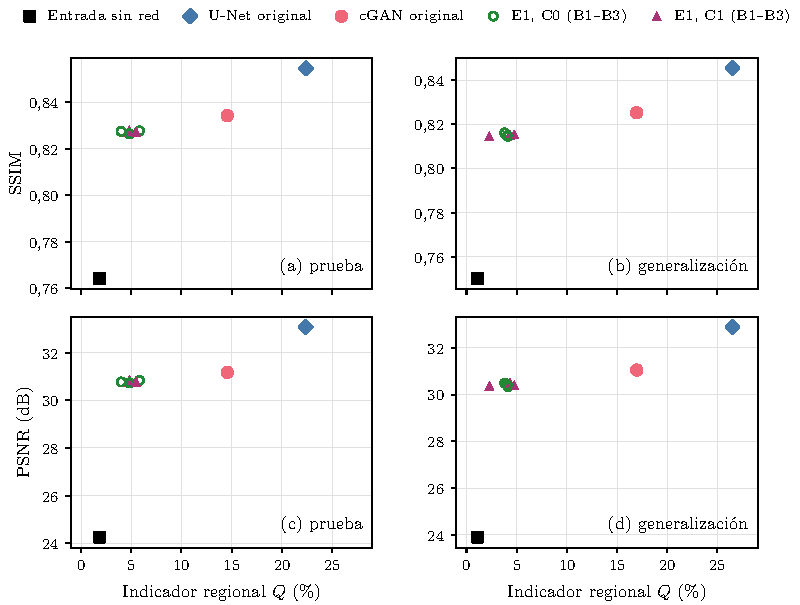
\includegraphics{fig4-4_compromiso.pdf}
\caption[Compromiso entre similitud de imagen y conservación de cuentas]{Compromiso entre similitud de imagen y conservación de cuentas en la evaluación final: SSIM (a, b) y PSNR (c, d) frente al indicador regional $Q$, en prueba (a, c) y en generalización (b, d). Cada símbolo es un macropromedio por partición; las seis variantes del ensayo de borde se muestran completas, sin seleccionar semillas. Evaluación descriptiva sobre datos potencialmente expuestos. Fuente: elaboración propia a partir de los resultados corregidos (C2) de la evaluación final en el repositorio de referencia.}
\label{fig:compromiso}
\end{figure}

La \cref{fig:comparacion-fija} ilustra estos resultados sobre imágenes concretas. Para no seleccionar casos favorables, se fijaron por índice la vista~0 y la realización~0 de cada geometría reservada, y los dieciséis paneles comparten una misma escala en el dominio normalizado de la \cref{eq:norm-v1}, sin ajustarla por imagen. La entrada al 5\,\% muestra el ruido de conteo, que es más visible en la roca; la U-Net produce imágenes suaves, con un oscurecimiento del interior del edificio coherente con su subestimación de las cuentas de la roca, y la cGAN conserva una textura más próxima a la de la referencia. Ninguna de esas apariencias constituye por sí sola evidencia de recuperación física: deben interpretarse junto con los indicadores regionales de la \cref{tab:res-ef01}.

\begin{figure}[htbp]
\centering
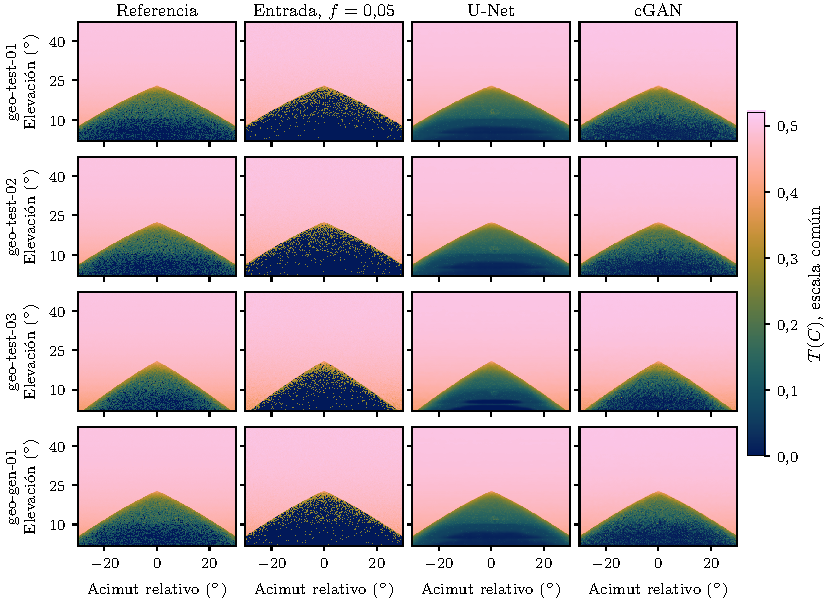
\includegraphics{fig4-7_comparacion_fija.pdf}
\caption[Comparación de imágenes en las cuatro geometrías reservadas]{Comparación de imágenes en las cuatro geometrías reservadas: referencia de alta estadística, entrada con $f=0{,}05$ y salidas de la U-Net y de la cGAN originales, para la vista~0 y la realización~0 de cada geometría, fijadas por índice. Todas las imágenes se representan en el dominio normalizado $T(C)$ de la \cref{eq:norm-v1}, con una escala común a los dieciséis paneles; las matrices se muestran a su resolución nativa de $256\times256$ píxeles, sin interpolación. Evaluación descriptiva sobre datos potencialmente expuestos. Fuente: elaboración propia a partir de las predicciones conservadas de la evaluación final, con la regla de selección del informe de la dirección.}
\label{fig:comparacion-fija}
\end{figure}

Para mostrar de forma explícita una limitación, la \cref{fig:caso-desfavorable} toma la geometría con el mayor indicador regional de la cGAN original entre las cuatro reservadas, geo-test-03, con un $Q$ de 27,835\,\%, y conserva la misma vista y realización. La regla se basa en el indicador agregado de la geometría y no en la búsqueda de la imagen visualmente más desfavorable. La figura incluye las seis continuaciones y los residuos de los nueve métodos respecto de la referencia, con una escala común y simétrica. El residuo de la entrada está dominado por el ruido de conteo de la roca, mientras que los de las redes tienen menor amplitud, pero no se anulan en el interior del edificio. Los residuos se expresan en $T(C)$ y no representan directamente sesgos de cuentas ni errores de densidad, y el valor de $Q$ citado corresponde a la geometría completa y no al panel mostrado. Esta comparación es posterior a la evaluación y tiene carácter ilustrativo.

\begin{figure}[htbp]
\centering
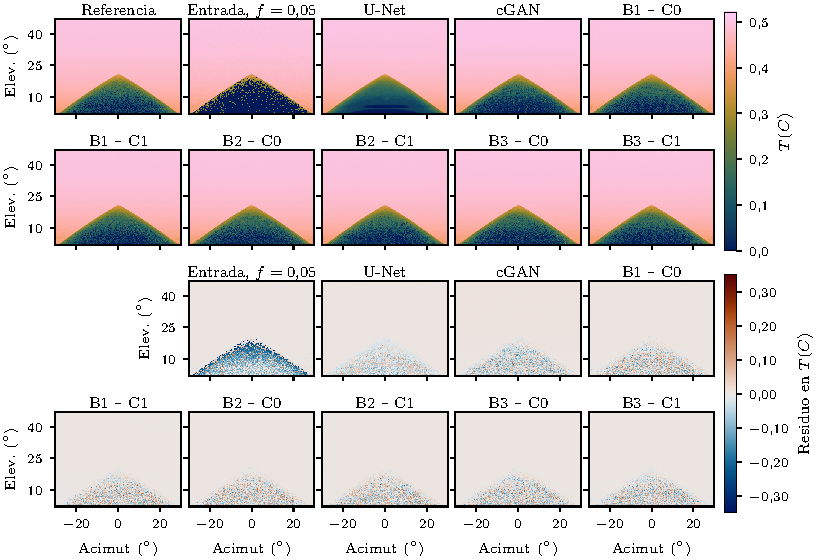
\includegraphics{fig4-8_caso_desfavorable.pdf}
\caption[Caso desfavorable: imágenes y residuos de todos los modelos]{Caso desfavorable de la evaluación final: geo-test-03, la geometría con el mayor indicador regional de la cGAN original ($Q=27{,}835\,\%$), vista~0 y realización~0. Filas superiores: referencia, entrada y salidas de las ocho redes en $T(C)$, con la escala común de la \cref{fig:comparacion-fija}. Filas inferiores: residuo de cada método respecto de la referencia en $T(C)$, con una escala común y simétrica de $\pm0{,}350$. Comparación posterior a la evaluación, seleccionada con una regla descriptiva explícita; evaluación descriptiva sobre datos potencialmente expuestos. Fuente: elaboración propia a partir de las predicciones conservadas de la evaluación final, con la regla de selección del informe de la dirección.}
\label{fig:caso-desfavorable}
\end{figure}

\subsection{Error de borde y contraste de las anomalías}
\label{subsec:res-regiones}

La reducción del error espacial de borde observada en validación se repitió en las cuatro geometrías reservadas y en las tres parejas, como muestra la \cref{fig:borde}. En prueba, el término de borde redujo ese error entre 3,7 y 4,7 puntos porcentuales y, en generalización, entre 3,7 y 4,0 puntos; en términos relativos, entre un 31 y un 40\,\% en las doce combinaciones de pareja y geometría. Con el término de borde, las continuaciones alcanzaron errores de borde de 6,6 a 8,3\,\%, comparables a los de la U-Net, de 6,7 a 7,2\,\%, y muy inferiores a los de la cGAN original, de 13,4 a 14,5\,\%, que fue el único método con un error de borde mayor que el de la entrada.

\begin{figure}[htbp]
\centering
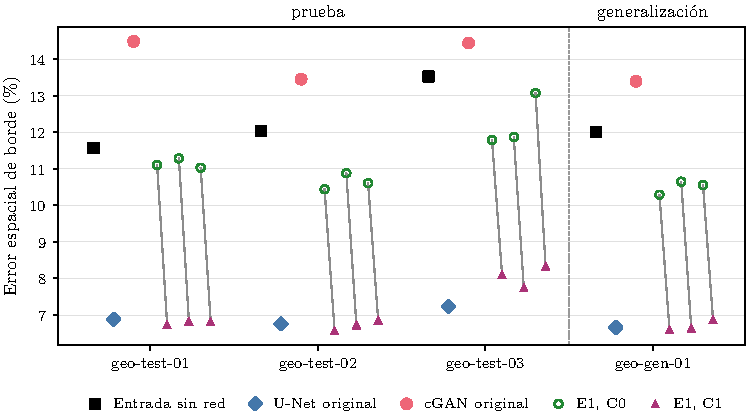
\includegraphics{fig4-5_borde.pdf}
\caption[Error espacial de borde por geometría en la evaluación final]{Error espacial de borde por geometría en la evaluación final. Para cada pareja B1--B3, el segmento une la variante C0, sin término de borde, con la variante C1, que lo incorpora. Evaluación descriptiva sobre datos potencialmente expuestos. Fuente: elaboración propia a partir de los resultados corregidos (C2) de la evaluación final en el repositorio de referencia.}
\label{fig:borde}
\end{figure}

La \cref{tab:contraste-c2} presenta el error de contraste antes y después de la corrección C2, sobre el soporte común de 30 combinaciones de anomalía y vista en prueba y de 16 en generalización. Todas las redes redujeron el error de contraste de la entrada, de 0,337 a entre 0,092 y 0,135 en prueba y de 0,290 a entre 0,072 y 0,115 en generalización, y la U-Net obtuvo el menor en ambas particiones. La corrección modificó los valores en menos de 0,005 en todos los casos salvo dos: la entrada en generalización, cuyo error pasó de 0,271327 a 0,289711, y una variante cuyo cambio altera la interpretación: en la pareja B1 sobre generalización, la variante C1 pasó de tener un error de contraste mayor que C0, de 0,137584 frente a 0,101319, a tener uno menor, de 0,090703 frente a 0,105524. Que una corrección numérica de la selección de controles invierta el signo de esa comparación indica que las diferencias de contraste entre variantes de una misma pareja, basadas en pocas combinaciones de una sola geometría, son sensibles a detalles del cálculo y no deben interpretarse como un efecto robusto del término de borde.

\begin{table}[htbp]
\centering
\caption[Error de contraste antes y después de la corrección C2]{Error absoluto medio de contraste (adimensional) en la evaluación final, con la selección original de controles y con la corrección numérica C2 de la selección de controles. Soporte común: 30 combinaciones de anomalía y vista en prueba y 16 en generalización. Fuente: elaboración propia a partir de la comparación antes y después de la revisión C2 en el repositorio de referencia.}
\label{tab:contraste-c2}
\small
\begin{tabular}{@{}lrrrr@{}}
\toprule
 & \multicolumn{2}{c}{Prueba} & \multicolumn{2}{c}{Generalización} \\
\cmidrule(lr){2-3}\cmidrule(l){4-5}
Método & Original & C2 & Original & C2 \\
\midrule
Entrada sin red & 0{,}336628 & 0{,}337054 & 0{,}271327 & 0{,}289711 \\
U-Net original & 0{,}093172 & 0{,}092463 & 0{,}072958 & 0{,}071503 \\
cGAN original & 0{,}135066 & 0{,}135104 & 0{,}088471 & 0{,}086302 \\
B1 -- C0 & 0{,}132899 & 0{,}133285 & 0{,}101319 & 0{,}105524 \\
B1 -- C1 & 0{,}100570 & 0{,}102743 & 0{,}137584 & 0{,}090703 \\
B2 -- C0 & 0{,}112721 & 0{,}112458 & 0{,}113495 & 0{,}114919 \\
B2 -- C1 & 0{,}108925 & 0{,}109112 & 0{,}099638 & 0{,}096729 \\
B3 -- C0 & 0{,}116936 & 0{,}116575 & 0{,}076043 & 0{,}073659 \\
B3 -- C1 & 0{,}127687 & 0{,}127915 & 0{,}077899 & 0{,}077246 \\
\bottomrule
\end{tabular}
\end{table}

\subsection{Comparaciones predeclaradas}
\label{subsec:res-comparaciones}

La \cref{tab:comparaciones} resume las doce comparaciones fijadas en el protocolo, seis por partición, con el número de geometrías en las que el candidato no empeoró cada métrica respecto de su comparador. Las doce se clasificaron como compromiso o deterioro conforme a la \cref{eq:clasificacion}, y ninguna cambió de clase con la corrección C2. La cGAN y la U-Net mejoraron el SSIM, el PSNR y el contraste de la entrada en todas las geometrías, pero aumentaron $Q$ en todas; la cGAN empeoró, además, los errores de cielo y de borde de la entrada. Frente a la U-Net, la cGAN solo mejoró $Q$. Dentro de las parejas del ensayo de borde, C1 mejoró los errores de cielo y de borde en todas las geometrías, mientras que $Q$, el contraste, el SSIM y el PSNR cambiaron de signo según la pareja y la geometría, con diferencias de SSIM no mayores de 0,002 y de PSNR no mayores de 0,12~dB. Ninguna clasificación implica significación ni superioridad estadística, y la elección de las semillas no se modificó después de abrir las particiones reservadas.

\begin{table}[htbp]
\centering
\caption[Comparaciones predeclaradas de la evaluación final]{Comparaciones predeclaradas de la evaluación final: número de geometrías en las que el candidato no empeoró cada métrica respecto del comparador (prueba: tres geometrías; generalización: una) y clasificación según la \cref{eq:clasificacion}. Fuente: elaboración propia a partir de los resultados corregidos (C2) de la evaluación final en el repositorio de referencia.}
\label{tab:comparaciones}
\footnotesize
\setlength{\tabcolsep}{4pt}
\begin{tabular}{@{}lrrrrrrl@{}}
\toprule
Comparación & SSIM & PSNR & $Q$ & Cielo & Borde & Contraste & Clase \\
\midrule
\multicolumn{8}{@{}l}{\emph{Prueba}} \\
cGAN frente a entrada & 3/3 & 3/3 & 0/3 & 0/3 & 0/3 & 3/3 & Compromiso o deterioro \\
U-Net frente a entrada & 3/3 & 3/3 & 0/3 & 3/3 & 3/3 & 3/3 & Compromiso o deterioro \\
cGAN frente a U-Net & 0/3 & 0/3 & 3/3 & 0/3 & 0/3 & 0/3 & Compromiso o deterioro \\
B1: C1 frente a C0 & 2/3 & 2/3 & 2/3 & 3/3 & 3/3 & 3/3 & Compromiso o deterioro \\
B2: C1 frente a C0 & 1/3 & 2/3 & 1/3 & 3/3 & 3/3 & 2/3 & Compromiso o deterioro \\
B3: C1 frente a C0 & 2/3 & 2/3 & 2/3 & 3/3 & 3/3 & 2/3 & Compromiso o deterioro \\
\midrule
\multicolumn{8}{@{}l}{\emph{Generalización}} \\
cGAN frente a entrada & 1/1 & 1/1 & 0/1 & 0/1 & 0/1 & 1/1 & Compromiso o deterioro \\
U-Net frente a entrada & 1/1 & 1/1 & 0/1 & 1/1 & 1/1 & 1/1 & Compromiso o deterioro \\
cGAN frente a U-Net & 0/1 & 0/1 & 1/1 & 0/1 & 0/1 & 0/1 & Compromiso o deterioro \\
B1: C1 frente a C0 & 0/1 & 1/1 & 0/1 & 1/1 & 1/1 & 1/1 & Compromiso o deterioro \\
B2: C1 frente a C0 & 1/1 & 1/1 & 0/1 & 1/1 & 1/1 & 1/1 & Compromiso o deterioro \\
B3: C1 frente a C0 & 0/1 & 0/1 & 1/1 & 1/1 & 1/1 & 0/1 & Compromiso o deterioro \\
\bottomrule
\end{tabular}
\end{table}

% =============================================================================
\section{Desempeño frente a la exposición (OE3)}
\label{sec:res-oe3}

Esta sección presenta el análisis descriptivo de la sección~\ref{subsec:met-factor}, que compara la entrada sin red con cuatro fracciones de conteo con las ocho redes evaluadas al 5\,\%. Como la evaluación final, se trata de un análisis posterior a la apertura de las reservas y sobre datos potencialmente expuestos, y no de una validación confirmatoria ni de una selección de modelos.

\subsection{Curvas descriptivas de exposición}
\label{subsec:res-curvas}

La \cref{tab:curvas} reúne las métricas de la entrada sin red con fracciones de 0,01, 0,05, 0,10 y 0,50 junto con las de las redes, y la \cref{fig:curvas} las representa frente a la fracción de conteos conservada. El caso de 0,05 reprodujo los valores de la entrada de la evaluación final con una tolerancia de $10^{-12}$. Como era de esperar, la calidad de la entrada mejoró de forma monótona con la fracción: en prueba, el SSIM pasó de 0,6959 al 1\,\% a 0,9250 al 50\,\%, el PSNR de 22,537 a 33,101~dB y $Q$ disminuyó de 2,897 a 0,437\,\%. El error de contraste se calculó sobre el soporte común a las cuatro fracciones y a las ocho redes, de 21 combinaciones en prueba y 11 en generalización, porque con la fracción 0,01 algunas realizaciones tienen controles sin cuentas; por ello, esos valores no son comparables con los de la \cref{tab:contraste-c2}.

\begin{table}[htbp]
\centering
\caption[Métricas de la entrada sin red con cuatro fracciones y de las redes al 5\,\%]{Métricas de la entrada sin red con cuatro fracciones de conteo y de las redes evaluadas con $f=0{,}05$. $Q$ en porcentaje de las cuentas de referencia; contraste sobre el soporte común de 21 combinaciones en prueba y 11 en generalización. Análisis descriptivo posterior sobre datos potencialmente expuestos. Fuente: elaboración propia a partir de las curvas descriptivas de exposición y de los resultados corregidos (C2) en el repositorio de referencia.}
\label{tab:curvas}
\small
\begin{tabular}{@{}lrrrr@{}}
\toprule
Método y fracción & SSIM & PSNR (dB) & $Q$ (\%) & Contraste \\
\midrule
\multicolumn{5}{@{}l}{\emph{Prueba}} \\
Entrada sin red, 1\,\% & 0{,}6959 & 22{,}537 & 2{,}897 & 0{,}504 \\
Entrada sin red, 5\,\% & 0{,}7643 & 24{,}258 & 1{,}832 & 0{,}164 \\
Entrada sin red, 10\,\% & 0{,}7964 & 25{,}722 & 1{,}334 & 0{,}111 \\
Entrada sin red, 50\,\% & 0{,}9250 & 33{,}101 & 0{,}437 & 0{,}034 \\
U-Net original, 5\,\% & 0{,}8545 & 33{,}074 & 22{,}388 & 0{,}070 \\
cGAN original, 5\,\% & 0{,}8342 & 31{,}170 & 14{,}566 & 0{,}077 \\
E1, seis variantes, 5\,\% & 0{,}8263--0{,}8278 & 30{,}729--30{,}849 & 3{,}996--5{,}825 & 0{,}065--0{,}074 \\
\midrule
\multicolumn{5}{@{}l}{\emph{Generalización}} \\
Entrada sin red, 1\,\% & 0{,}6851 & 22{,}299 & 3{,}067 & 0{,}569 \\
Entrada sin red, 5\,\% & 0{,}7502 & 23{,}904 & 1{,}093 & 0{,}159 \\
Entrada sin red, 10\,\% & 0{,}7834 & 25{,}349 & 0{,}895 & 0{,}119 \\
Entrada sin red, 50\,\% & 0{,}9197 & 32{,}752 & 0{,}449 & 0{,}040 \\
U-Net original, 5\,\% & 0{,}8454 & 32{,}883 & 26{,}505 & 0{,}066 \\
cGAN original, 5\,\% & 0{,}8252 & 31{,}047 & 16{,}959 & 0{,}079 \\
E1, seis variantes, 5\,\% & 0{,}8145--0{,}8161 & 30{,}331--30{,}509 & 2{,}271--4{,}755 & 0{,}067--0{,}095 \\
\bottomrule
\end{tabular}
\end{table}

\begin{figure}[htbp]
\centering
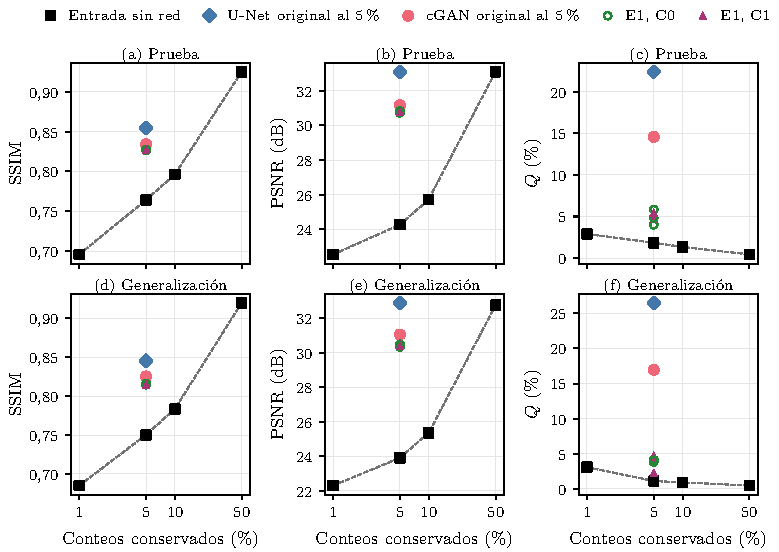
\includegraphics{fig4-6_curvas_exposicion.pdf}
\caption[Curvas descriptivas de exposición de la entrada sin red]{Curvas descriptivas de exposición: SSIM, PSNR e indicador regional $Q$ de la entrada sin red con cuatro fracciones de conteo, en prueba (a--c) y en generalización (d--f), junto con las ocho redes, evaluadas solo con la fracción 0,05. Las líneas discontinuas unen valores medidos como guía visual y no se usan para interpolar factores de adquisición. Análisis descriptivo posterior sobre datos potencialmente expuestos. Fuente: elaboración propia a partir de las curvas descriptivas de exposición y de los resultados corregidos (C2) en el repositorio de referencia.}
\label{fig:curvas}
\end{figure}

En prueba, la cGAN original al 5\,\% obtuvo un SSIM de 0,8342 y un PSNR de 31,170~dB, superiores a los de la entrada sin red al 10\,\%, de 0,7964 y 25,722~dB. La \cref{tab:cgan-10} muestra que esa relación no depende del promedio: se cumplió en cada una de las cuatro geometrías reservadas, tanto en SSIM como en PSNR, mientras que en todas ellas la cGAN quedó por debajo de la entrada al 50\,\%. Ambas métricas comparan cada imagen con la misma referencia de alta estadística, de modo que no comparan directamente la salida de la red con la entrada al 10\,\%. Sin embargo, $Q$ pasó de 1,334\,\% en esa entrada a 14,566\,\% en la cGAN: la mejora de similitud no implicó conservar mejor las cuentas.

\begin{table}[htbp]
\centering
\caption[cGAN al 5\,\% frente a la entrada sin red al 10\,\% por geometría]{SSIM y PSNR de la cGAN original con $f=0{,}05$ y de la entrada sin red con el 10\,\% de los conteos, por geometría reservada; ambas métricas se calculan frente a la misma referencia de alta estadística. Análisis descriptivo posterior sobre datos potencialmente expuestos. Fuente: elaboración propia a partir de los resultados corregidos (C2) y de las curvas descriptivas de exposición en el repositorio de referencia.}
\label{tab:cgan-10}
\small
\begin{tabular}{@{}lrrrr@{}}
\toprule
 & \multicolumn{2}{c}{SSIM} & \multicolumn{2}{c}{PSNR (dB)} \\
\cmidrule(lr){2-3}\cmidrule(l){4-5}
Geometría & cGAN, 5\,\% & Entrada, 10\,\% & cGAN, 5\,\% & Entrada, 10\,\% \\
\midrule
geo-test-01 & 0{,}8095 & 0{,}7667 & 30{,}900 & 25{,}240 \\
geo-test-02 & 0{,}8233 & 0{,}7822 & 31{,}107 & 25{,}468 \\
geo-test-03 & 0{,}8697 & 0{,}8403 & 31{,}504 & 26{,}458 \\
geo-gen-01 & 0{,}8252 & 0{,}7834 & 31{,}047 & 25{,}349 \\
\bottomrule
\end{tabular}
\end{table}

 Las seis continuaciones también superaron, en estos promedios, el SSIM y el PSNR de la entrada al 10\,\%, con un $Q$ de entre 3,996 y 5,825\,\% frente al 1,334\,\%, y la U-Net ofreció los mayores valores de similitud con el mayor $Q$. En los macropromedios de prueba, las ocho redes quedaron entre los valores de la entrada al 10 y al 50\,\% tanto en SSIM como en PSNR. En generalización ocurrió lo mismo, salvo que el PSNR de la U-Net superó ligeramente el de la entrada al 50\,\%, con 32,883 frente a 32,752~dB, aunque su SSIM permaneció por debajo. En contraste, las redes, con errores de 0,065 a 0,095, quedaron entre la entrada al 10\,\% y al 50\,\%. Estas diferencias no constituyen una prueba de superioridad estadística, porque las realizaciones de una misma geometría no se trataron como geometrías independientes, y los cruces por geometría de los demás modelos, que el análisis también registró, no deben sustituirse por los promedios.

\subsection{Razones nominales de exposición y alcance del factor de reducción}
\label{subsec:res-factor}

Según la \cref{eq:factor}, una red alimentada con $f_{\mathrm{mod}}=0{,}05$ y una entrada sin red con fracción $f_{\mathrm{ent}}$ guardan una razón nominal de exposiciones $R=f_{\mathrm{ent}}/0{,}05$, que vale 2 frente a la entrada al 10\,\%, 10 frente a la del 50\,\% y 20 frente a la referencia completa. Con esa equivalencia, los resultados anteriores indican que las redes al 5\,\% superan en SSIM y PSNR a una entrada con el doble de conteos, en el caso de la cGAN en cada una de las cuatro geometrías, con deterioro de la conservación regional de las cuentas, y que no alcanzan, salvo el PSNR de la U-Net en generalización, a la entrada con diez veces más conteos. La rejilla sitúa, por tanto, los cruces de las métricas de similitud entre los puntos asociados nominalmente a 2 y a 10; en el PSNR de la U-Net en generalización, el cruce queda fuera de la rejilla y no se extrapoló.

Estos resultados no permiten estimar un factor de reducción entre 2 y 10, un factor máximo alcanzable ni un intervalo de confianza, porque no hay mediciones intermedias, no se adoptó ninguna ley de interpolación y las redes solo se evaluaron con la fracción de 0,05. Tampoco el factor nominal de 20 asociado a $f=0{,}05$ es un factor alcanzado: describe la reducción de conteos de la entrada, no la calidad del resultado. Determinar el factor alcanzable exige un criterio de calidad aceptable, justificado por la aplicación o por una referencia científica externa, que separe la equivalencia descriptiva según SSIM y PSNR de la aceptación física según cuentas y contraste; como no se había fijado un criterio de calidad aceptable con un margen fundamentado, los resultados se informan como una comparación descriptiva por métrica, sin un factor único que oculte el deterioro de la conservación de cuentas, y el factor de reducción alcanzable no está demostrado. Las razones se refieren, además, a fracciones de conteos obtenidas por adelgazamiento de referencias idealizadas, y no a tiempos de adquisición medidos.

\subsection{Discusión}
\label{subsec:res-discusion-oe2}

Se implementó y entrenó un modelo generativo condicionado para recuperar imágenes muográficas a partir de una fracción de conteos de 0,05, y se comparó con una red U-Net entrenada con pérdida L1 y con la entrada de baja estadística escalada a cuentas equivalentes. La evaluación final incluyó tres geometrías de prueba y una de generalización, con seis vistas y veinte realizaciones por vista, y ocho redes previamente congeladas, entre ellas seis continuaciones destinadas a estudiar la conservación regional y el error de borde; estas continuaciones comparten la inicialización y no constituyen entrenamientos independientes desde cero.

El resultado central es un compromiso entre la similitud visual y la conservación de las cuentas. Todas las redes redujeron el ruido de conteo y aumentaron el SSIM y el PSNR de la entrada en las cuatro geometrías reservadas, pero ninguna mejoró todos los indicadores a la vez: las que más se acercaron a la referencia en esas métricas, la U-Net y, en menor medida, la cGAN, fueron también las que más desplazaron las cuentas de la roca y de las anomalías. La U-Net, entrenada solo con el término L1, superó a la cGAN original en SSIM y en PSNR en las dos particiones, de modo que la componente antagónica no mostró una ventaja global en esta comparación; atribuirle una recuperación física superior requeriría una evidencia que estos resultados no proporcionan. La entrada escalada, en cambio, conservó mejor los promedios regionales pese a su ruido visible, lo que es coherente con la esperanza condicional del adelgazamiento binomial (\cref{eq:pares-media}), sin que ello implique precisión en cada píxel o realización. Este comportamiento es coherente con el compromiso entre distorsión y percepción descrito en la literatura de restauración de imágenes, según el cual las métricas de distorsión y la fidelidad a la distribución de los datos no pueden optimizarse simultáneamente sin límite \parencite{blau2018}, y con el hecho de que el SSIM y el PSNR se calcularon en una escala logarítmica normalizada, en la que reducir las fluctuaciones píxel a píxel mejora ambas métricas aunque se desplace la cuenta media de una región \parencite{hore2010}. Una explicación compatible con el diagnóstico del piloto es que la reconstrucción tiende a atenuar los extremos de la escala logarítmica, lo que se traduce en una subestimación de las regiones de menor conteo, como las cavidades y el cuerpo denso; esa explicación no se sometió a una prueba específica.

Los ajustes acotaron, pero no resolvieron, ese compromiso. El término regional redujo el sesgo de cuentas, aunque con una magnitud dependiente de la semilla y con deterioro del error espacial, porque restringe la cuenta media de cada región y no su distribución interna. El término espacial de borde corrigió de forma consistente la transición entre roca y cielo, en validación y en las cuatro geometrías reservadas, pero no produjo una mejora simultánea de todos los indicadores y dejó sin resolver el sesgo del interior de geo-val-01. Las doce comparaciones predeclaradas conservaron la clasificación de compromiso o deterioro en al menos un indicador, y no se seleccionó una semilla favorable después de abrir los datos de prueba. La corrección numérica C2 estabilizó la selección de los controles de contraste y conservó sus índices exactos; el SSIM, el PSNR y los indicadores regionales permanecieron iguales, y su efecto sobre el contraste, incluida la inversión de la comparación de la pareja B1 en generalización, se informó con las tablas corregidas y su comparación con el cálculo original.

Se verificaron, por tanto, la implementación, el entrenamiento y la evaluación descriptiva con el 5\,\% de los conteos. La mejora de la similitud y la reducción del ruido no demuestran por sí solas la equivalencia con la alta estadística, porque persisten alteraciones de las cuentas y no se había fijado un margen físico de equivalencia. El alcance se limita a referencias idealizadas y a un catálogo conocido, con exposición histórica de las escenas reservadas. Por ello, no se afirma la generalización a volcanes reales, la equivalencia física, el desempeño con otras fracciones de conteo ni la validación experimental de un factor de reducción del tiempo de adquisición. En el análisis de exposición, la conclusión válida es descriptiva: las redes al 5\,\% superan determinadas métricas de una entrada con el doble de conteos, con deterioro de otros indicadores; convertir ese resultado en una equivalencia física, en una reducción efectiva de 20 veces o en una afirmación sobre el desempeño del modelo con el 1, el 10 o el 50\,\% de los conteos no es válido con la evidencia disponible.
